\documentclass[12pt]{article}


%Utilize aqui os seus pacotes preferidos para auxilair na escrita do documento

\usepackage{sbc-template}
\usepackage{graphicx}
\usepackage{url}
\usepackage[brazil]{babel} 
\usepackage[utf8]{inputenc}
\usepackage{booktabs}
\usepackage[pdftex]{hyperref}
\usepackage{indentfirst}
\usepackage{float}
\usepackage{graphicx,color}
\usepackage[linesnumbered]{algorithm2e}
\usepackage{array}
\usepackage{url}

     
\sloppy

\title{Título do Trabalho: Subtítulo}

\author{Nome do Autor Um\inst{1}, Nome do Autor Dois\inst{1}, \\Nome do Autor Três\inst{1}, Nome do Autor Quatro\inst{1}, \\Nome do Autor N. \inst{1}, Nome do Coorientador\inst{2}, Nome do Orientador\inst{2} } 

\address{Departamento de Computação (DCOMP)\\ Universidade Federal de Sergipe
  (UFS)\\
  Av. Marechal Rondon, s/n -- Jardim Rosa Elze -- CEP 49100-000 \\São Cristóvão -- SE -- Brazil \nextinstitute
  Programa de Pós-Graduação em Ciência da Computação - (PROCC)\\Universidade Federal de Sergipe
  (UFS)\\
  Av. Marechal Rondon, s/n -- Jardim Rosa Elze -- CEP 49100-000 \\São Cristóvão -- SE -- Brazil
  \email{autor01@dcomp.ufs.br, autor02@dcomp.ufs.br}
  \email{autor03@dcomp.ufs.br, autor04@dcomp.ufs.br}
  \email{autorn@dcomp.ufs.br, orientador@dcomp.ufs.br}
}

\begin{document} 

\maketitle

\begin{abstract}
\textbf {Context:} Appear the work context. \textbf {Objective:} This work aims to ... \textbf {Method:} Describe the methodological procedures used in the research. \textbf {Results:} Discuss the results of this work. \textbf {Conclusions:} Show the conclusions that were found.
\end{abstract}
     
\begin{resumo} 
  \textbf{Contexto:} Aparentar o contexto do trabalho. \textbf{Objetivo:} Este trabalho tem como objetivo ... \textbf{Método:} Descrever os procedimentos metodológicos utilizados na pesquisa. \textbf{Resultados:} Discutir sobre os resultados advindos deste trabalho. \textbf{Conclusões:} Mostrar as conclusões que foram encontradas.
\end{resumo}


\section{Introdução} 
\label{sec:introducao}

Explicar o por quê do projeto ser feito e especificar melhor nas subseções abaixo.

\subsection{Contextualização} 
\label{subsec:contextualizacao}
Contextualização... 1 parágrafo;
Problemática ... 1 parágrafo;

\subsection{Justificativa} 
Justificativa ... 1 parágrafo;

\subsection{Objetivos} 
Objetivos... 1 parágrafo;

\subsection{Benefícios} 

Benefícios... 1 parágrafo;

\subsection{Descrição das próximas seções} 
Descrição das próximas seções do trabalho ... 1 parágrafo.


\section{O que será feito? } \label{sec:oque}

Breve descrição das próximas subseções...

\subsection{Produto}

Descrição do Produto...

\subsection{Requisitos}

Descrição dos Requisitos...
Pode-se utilizar de recursos de Engenharia de Software \cite{pressman2021engenharia}.

\subsection{Modelagem dos Processos de negócio }

Descrição da modelagem dos processos de negócio do projeto...

Apresentar a modelagem do processo de negócio...


Apresentar As telas referente aos fluxos dos processos de negócio;

Obs.: Inclua Figuras, Tabelas, Quadros, Códigos, etc...


A \autoref{fig:fluxo_submissao} apresenta um fluxo descrevendo o processo principal de submissão um resumo científico para participação no Encontro de Iniciação Científica.

\begin{figure}[!htb]
\caption{Fluxo principal de submissão de resumo}
\label{fig:fluxo_submissao}
\centering
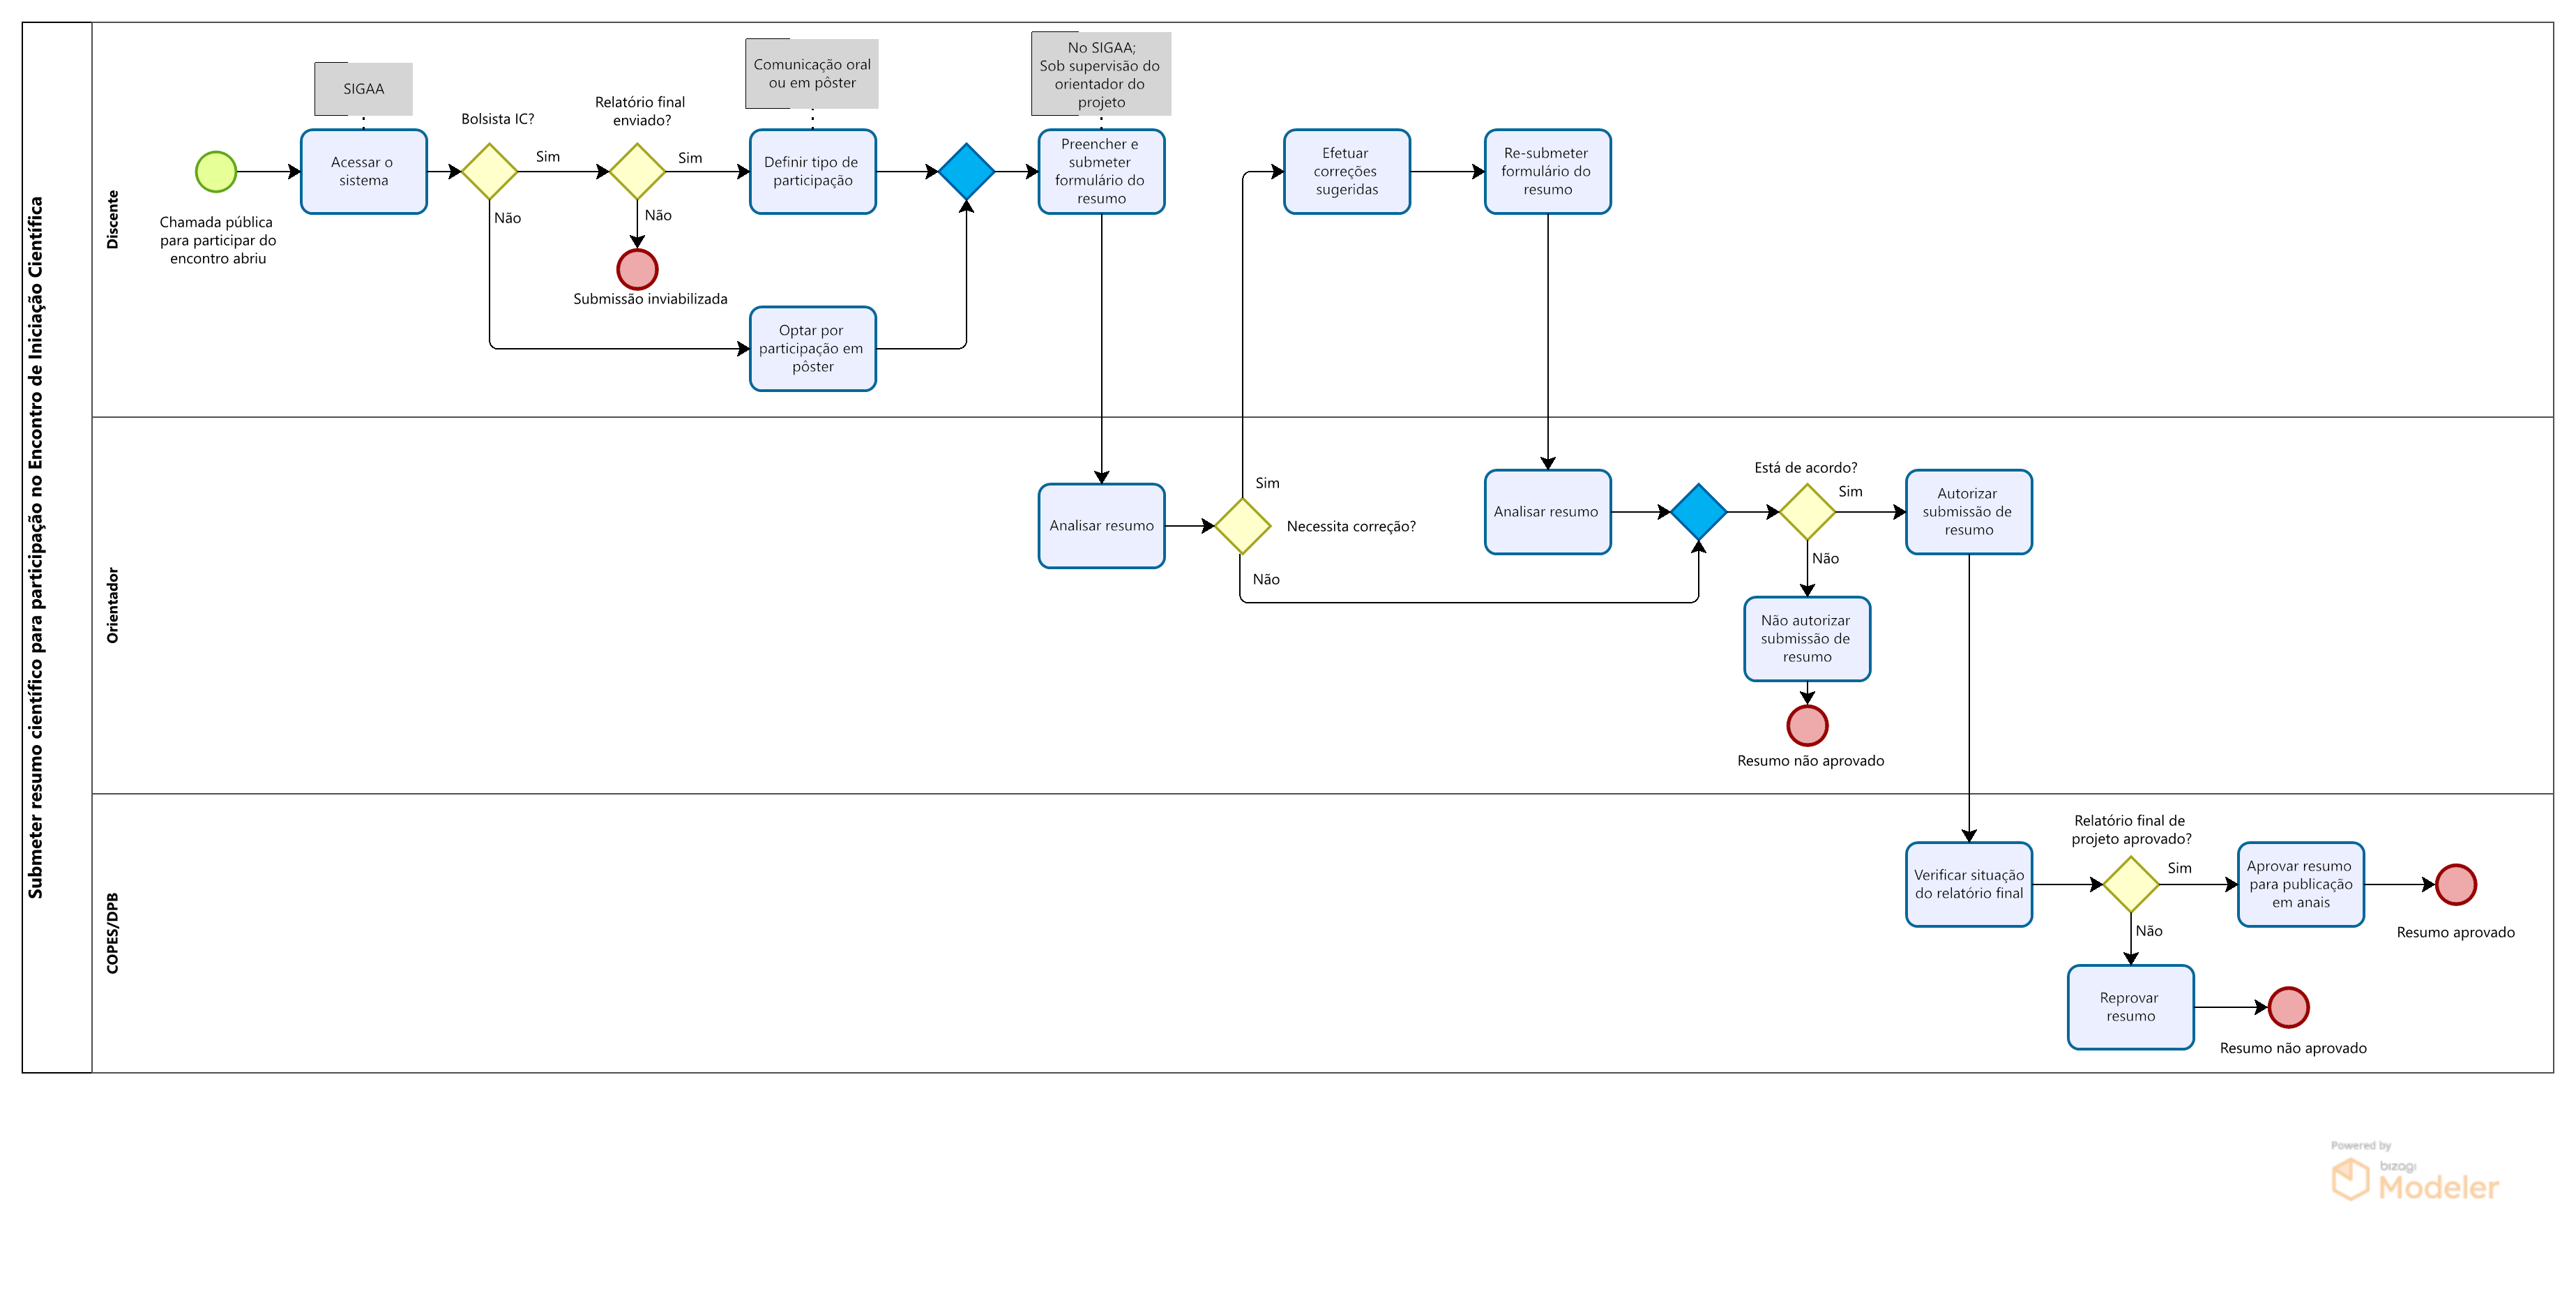
\includegraphics[width=12cm]{images/submeter-resumo-cientifico.png}
%\legend {Fonte: \url{https://shre.ink/9xnr}}
\end{figure}


\subsection{Telas do Sistema}

Apresentar As telas referente aos fluxos dos processos de negócio;

Obs.: Inclua Figuras, Tabelas, Quadros, Códigos, etc...


A Figura \autoref{fig:telas_sistema} apresenta as telas do Sistema Caixa Postal UFS.

\begin{figure}[H]
\caption{Telas do Sistema Caixa Postal UFS}
\label{fig:telas_sistema}
\centering
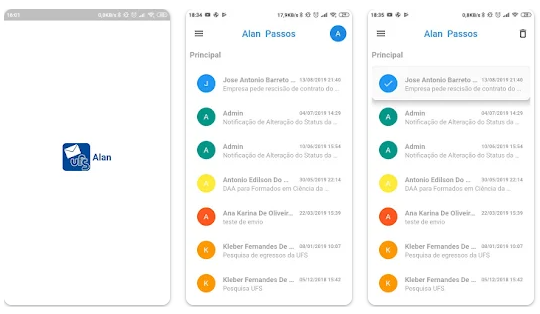
\includegraphics[width=12cm]{images/telas_caixa_postal_ufs.png}
%\legend {Fonte: \url{https://play.google.com/store/apps/details?id=br.ufs.nti.cxmobile}}
\end{figure}


\section{Quem fará o projeto}\label{sec:quem}

Breve descrição das próximas subseções...

\subsection{Stakeholders e Fatores Externos}
parceiros externos necessários para alcançar as metas.

\subsection{Equipe}
Apresentar a Equipe e a funão de cada um

\begin{itemize}
  \item Nome do Autor Um: Pesquisa, correções e escrita do manuscrito;
  \item Nome do Autor Dois: Pesquisa, correções e escrita do manuscrito;
  \item Nome do Autor Três: Pesquisa, correções e escrita do manuscrito;
  \item Nome do Autor Quatro: Pesquisa, correções e escrita do manuscrito;
  \item Nome do Autor N: Pesquisa, correções e escrita do manuscrito;
  \item Nome do Orientador: Coordenação do trabalho, correções e direcionamentos da pesquisa.
\end{itemize}

\section{Como o projeto será feito?} \label{sec:Como}
Breve descrição das próximas subseções...


\subsection{Premissas}

\subsection{Grupo de entregas}

\subsection{Restrições}


\section{Quando e quanto?} \label{sec:quandoquanto}
Breve descrição das próximas subseções...




\subsection{Riscos}

\subsection{Linha do tempo}


A \autoref{fig:linha_tempo} apresenta a linha do tempo planejada para o projeto.

\begin{figure}[H]
\caption{Linha do tempo planejada para o projeto}
\label{fig:linha_tempo}
\centering
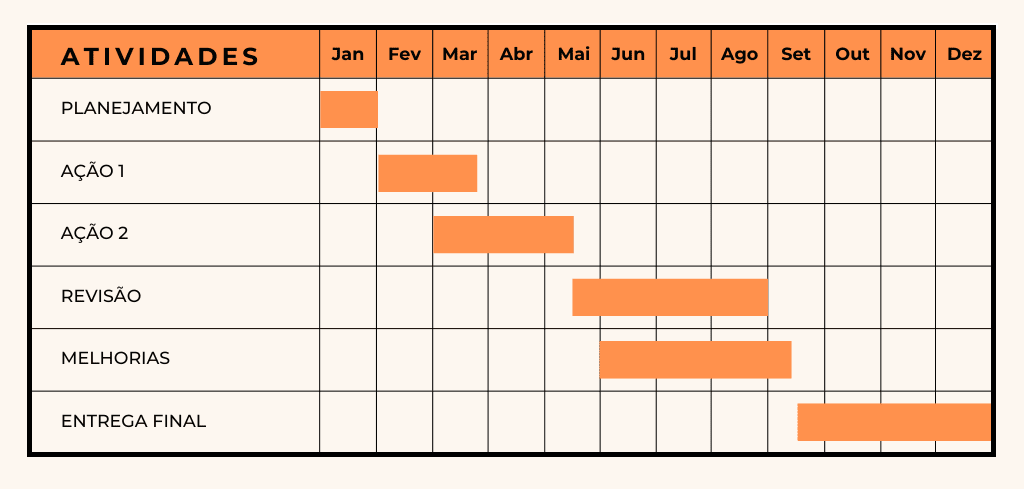
\includegraphics[width=12cm]{images/cronograma_projeto.png}
%\legend {Fonte: \url{https://www.voitto.com.br/blog/artigo/o-que-e-cronograma}}
\end{figure}



\subsection{Custos}


\section{Canvas do Projeto} 
\label{sec:pmc_projeto}

A \autoref{fig:pmc_projeto} apresenta o quadro do modelo de projeto \cite{finocchio2013project}, do inglês \textit{Project Model Canvas} (PMC) do projeto.

\begin{figure}[H]
\caption{Quadro do modelo de projeto}
\label{fig:pmc_projeto}
\centering
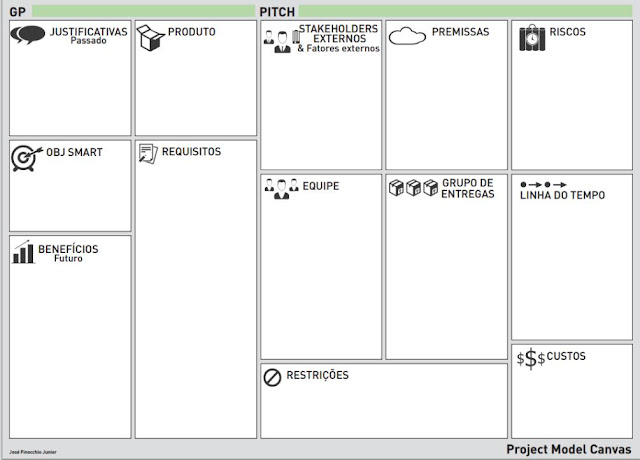
\includegraphics[width=12cm]{images/project_model_canva.jpg}
%\legend {Fonte: \url{https://www.voitto.com.br/blog/artigo/o-que-e-cronograma}}
\end{figure}



\section{Limitações do Trabalho} \label{sec:ameacas}

Inserir informações a cerca do que não foi apresentado no trabalho.



\section{Considerações Finais e Trabalhos Futuros} \label{sec:consideracoes}
Descrição das atividades realizadas para atingir o objetivo do trabalho... 2 paragrafo\\
Descrição da metodologia utilizada para atingir o objetivo do trabalho... 1 paragrafo\\
Descrição dos pontos fracos ou que possam inviabilizar a credibilidade do trabalho... 1 paragrafo\\
Descrição das atividades futuras para se concluir o trabalho... 1 paragrafo\\

\section*{Agradecimentos} \label{sec:agradecimentos}

Esta seção tem como objetivo agradecer a todas as pessoas e instituições que ajudaram na pesquisa, mas que não se qualificam para autoria.

Alguns periódicos e eventos exigem que sejam informados os dados refentes ao às organizações que financiaram a pesquisa.







\bibliographystyle{sbc}
\bibliography{referencias}

\end{document}
